%%    _____  _____
%%   |  __ \|  __ \    AUTHOR: Pedro Rivero
%%   | |__) | |__) |   ---------------------------------
%%   |  ___/|  _  /    DATE: November 10, 2021
%%   | |    | | \ \    ---------------------------------
%%   |_|    |_|  \_\   https://github.com/pedrorrivero
%%

\section{The NJL model}

%% ----------------------------------------------------------------------------
%% ----------------------------------------------------------------------------

\begin{frame}[allowframebreaks]{The Nambu--Jona-Lasino model (NJL)}

	An important path forward is to develop methods to simulate these models on quantum computers. This effort is only just beginning, however, it has only been achieved for relatively simple problems.

	\medskip

	\begin{itemize}
		\item<2-> \textbf{Nambu--Jona-Lasino model} (NJL) in $1+1$ dimensions: an effective field theory, regarded as a low-energy approximation to QCD.
    \item<2-> Originally developed pre-QCD to describe nucleons via an effective two-body point interaction. Nowadays gets reinterpreted as a theory of quarks.
    \item<2-> Inspired by the \textbf{BCS theory of superconductivity}.
		\item<3-> It retains certain key features of QCD, such as the so called Goldstone modes and \textbf{dynamical chiral symmetry breaking}; which in turn is responsible for the creation of dressed mass.
		\item<4-> This model can be solved nonperturbatively through the standard leading order truncation; an important characteristic since verifying the solutions returned by any quantum computation is currently a major challenge.
	\end{itemize}

%% ----------------------------------------------------------------------------
\break
%% ----------------------------------------------------------------------------

	The NJL \textbf{Lagrangian density} that we will make use of looks like:

	\begin{gather*}
		\mathcal{L}(x) =
	    \bar{\psi}_{\alpha}(x)
	    \qty(\delta_{\alpha\beta}i\slashed{\partial}-\hat{m}_{\alpha\beta})
	    \psi_{\beta}(x) + \mathcal{L}_{I}(x) \\[1em]
		\mathcal{L}_{I}(x) =
	    \frac{1}{2} G_{\pi} \qty[\bar{\psi}_{\alpha}(x)\psi_{\alpha}(x)]^2
	\end{gather*}

	From this expression for the Lagrangian density we can obtain the corresponding \textbf{Hamiltonian density} through the Legendre transform. In special, for $1+1$ dimensions:

	\begin{align*}
		\mathcal{H} \,=\,\,
	  & -\frac{i}{2} \bar{\psi}_{\alpha} \gamma^{1}
	    \qty(\partial_{1} \psi_{\alpha}) +
	    \frac{i}{2} \qty(\partial_{1}\bar{\psi}_{\alpha})\gamma^{1}\psi_{\alpha} +
	    \bar{\psi}_{\alpha} \hat{m}_{\alpha\beta} \psi_{\beta} -
	    \frac{1}{2} G_{\pi} \qty(\bar{\psi}_{\alpha}\psi_{\alpha})^{2}
	\end{align*}

\end{frame}


%% ----------------------------------------------------------------------------
%% ANALYTICAL SOLUTION
%% ----------------------------------------------------------------------------

\subsection{Analytical solution}

%% ----------------------------------------------------------------------------
%% ----------------------------------------------------------------------------

\begin{frame}[allowframebreaks]{Dressed mass and the gap equation}

  \vspace{-1em}
	\begin{multicols}{2}

		The \textbf{bare and dressed masses} appear on the bare quark propagator $S_{0}$, and the NJL dressed quark propagator $S$ respectively:

		\vspace{1em}

		\begin{gather*}
		  S_0^{-1} \defeq \slashed{p} - m + i\varepsilon \\[.5em]
		  S^{-1} \equiv S^{-1}_\text{\tiny NJL} \defeq \slashed{p} - M + i\varepsilon
		\end{gather*}

		\columnbreak

		\begin{center}
			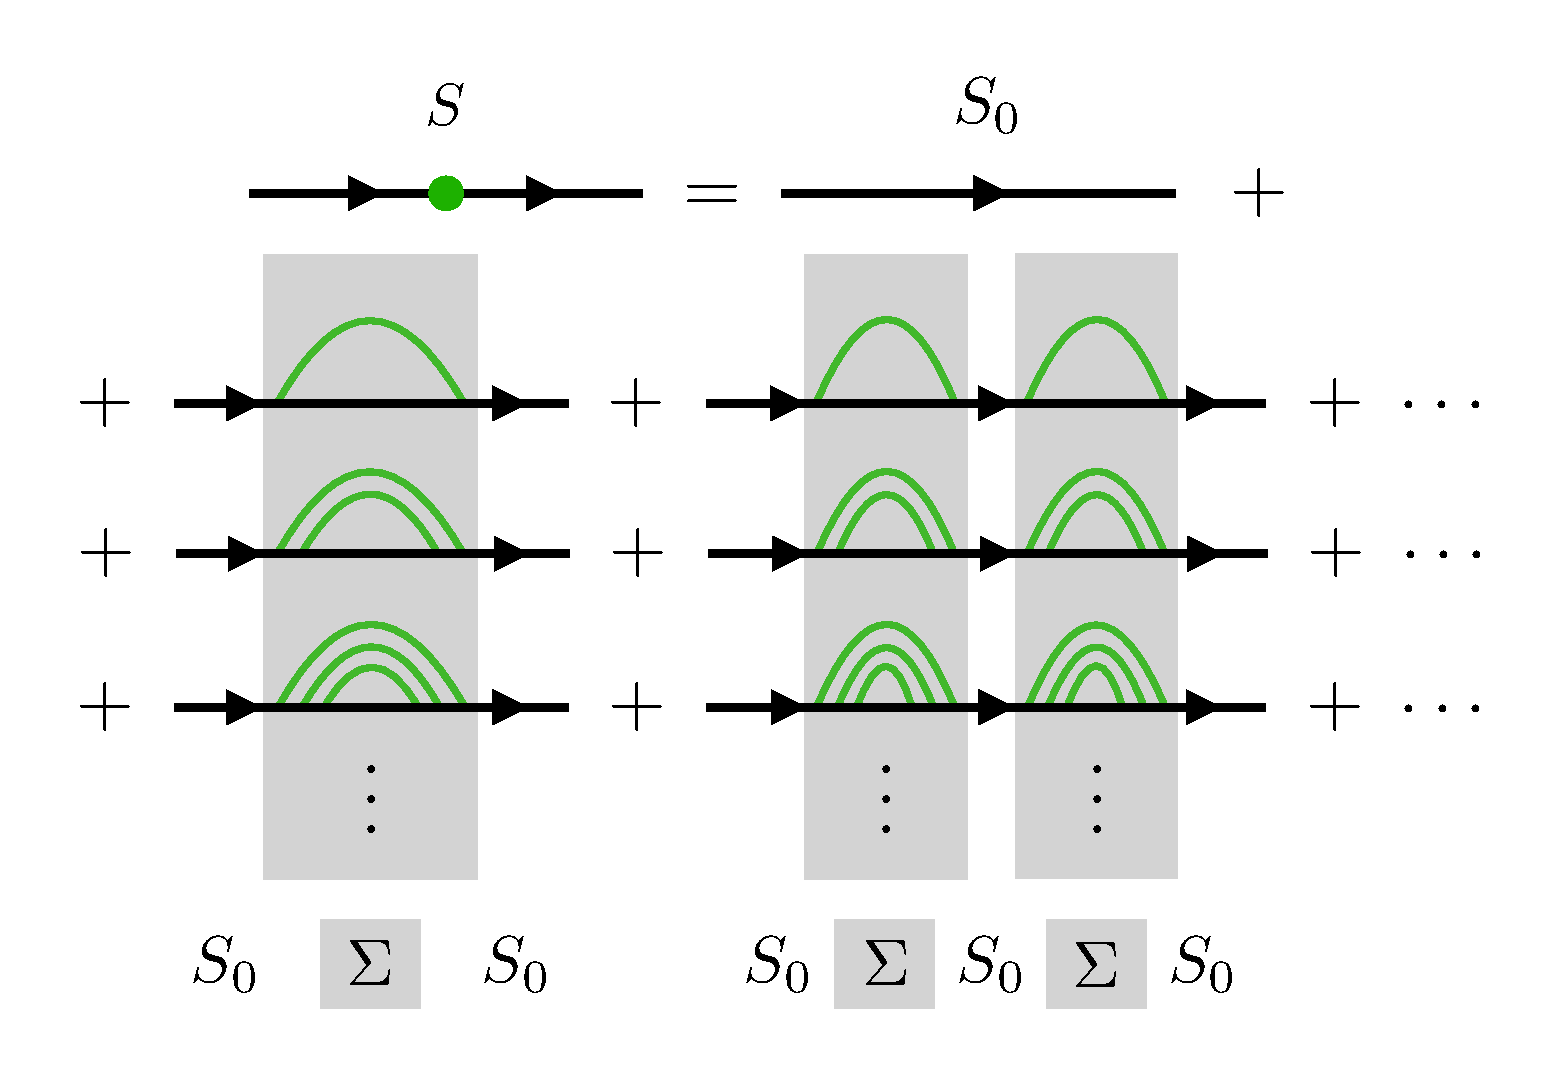
\includegraphics[width=.30\paperwidth]{Figures/chapter02/gap-equation}
		\end{center}

	\end{multicols}
  \vspace{-1em}

	We can find a relationship between these two by solving the \textbf{gap equation}:

	\begin{gather*}
		S^{-1} =
	    S_{0}^{-1} - 2iG_{\pi} \int \frac{\dd[2]{p}}{\qty(2\pi)^{2}}
	    N_\text{color} N_\text{flavor} \text{Tr}_\text{\tiny{D}}\qty[S] \\
	  M \simeq
	    m + 4iG_\pi N_\text{color} N_\text{flavor}
	    \int \frac{\dd[2]{p}}{(2\pi)^2} \frac{M}{p^2 - M^2}
	\end{gather*}

%% ----------------------------------------------------------------------------
\break
%% ----------------------------------------------------------------------------

	% To solve this last expression we first perform a \textbf{Wick rotation} $p_0 \ra i p_2 \qRa (p_0)^2 \ra - (p_2)^2$, followed by a transformation to \textbf{polar coordinates}:
  %
	% \begin{gather*}
	% 	M \simeq
	%     m + N_\text{color}  N_\text{flavor}
	%     \frac{G_\pi}{\pi} \int_{0}^{\infty} \frac{M}{p_E^2 + M^2} \dd{p_E^2}
	% \end{gather*}
  %
	% Finally, to make the integral converge, we introduce \textbf{proper time regularization}:
  %
	% \begin{gather*}
	%   \frac{1}{x^n} =
	%     \frac{1}{(n-1)!} \int_{0}^{\infty} \dd{\tau} \tau^{n-1} \exp[-\tau x] \ra
	%     \frac{1}{(n-1)!} \int_{1/\Lambda_{UV}^2}^{1/\Lambda_{IR}^2}
	%       \dd{\tau} \tau^{n-1} \exp[-\tau x] \\[5pt]
	%   M \simeq
	%     m + M N_\text{color} N_\text{flavor} \frac{G_\pi}{\pi}
	%     \int_{1/\Lambda_{UV}^2}^{1/\Lambda_{IR}^2} \frac{\dd{\tau}}{\tau}
	%     \exp[-\tau M^{2}]
	% \end{gather*}
  %
	% Where $\Lambda_{IR}$ and $\Lambda_{UV}$ are the \textbf{infrared and ultraviolet cutoffs} respectively.

%% ----------------------------------------------------------------------------
\break
%% ----------------------------------------------------------------------------

	\begin{center}
		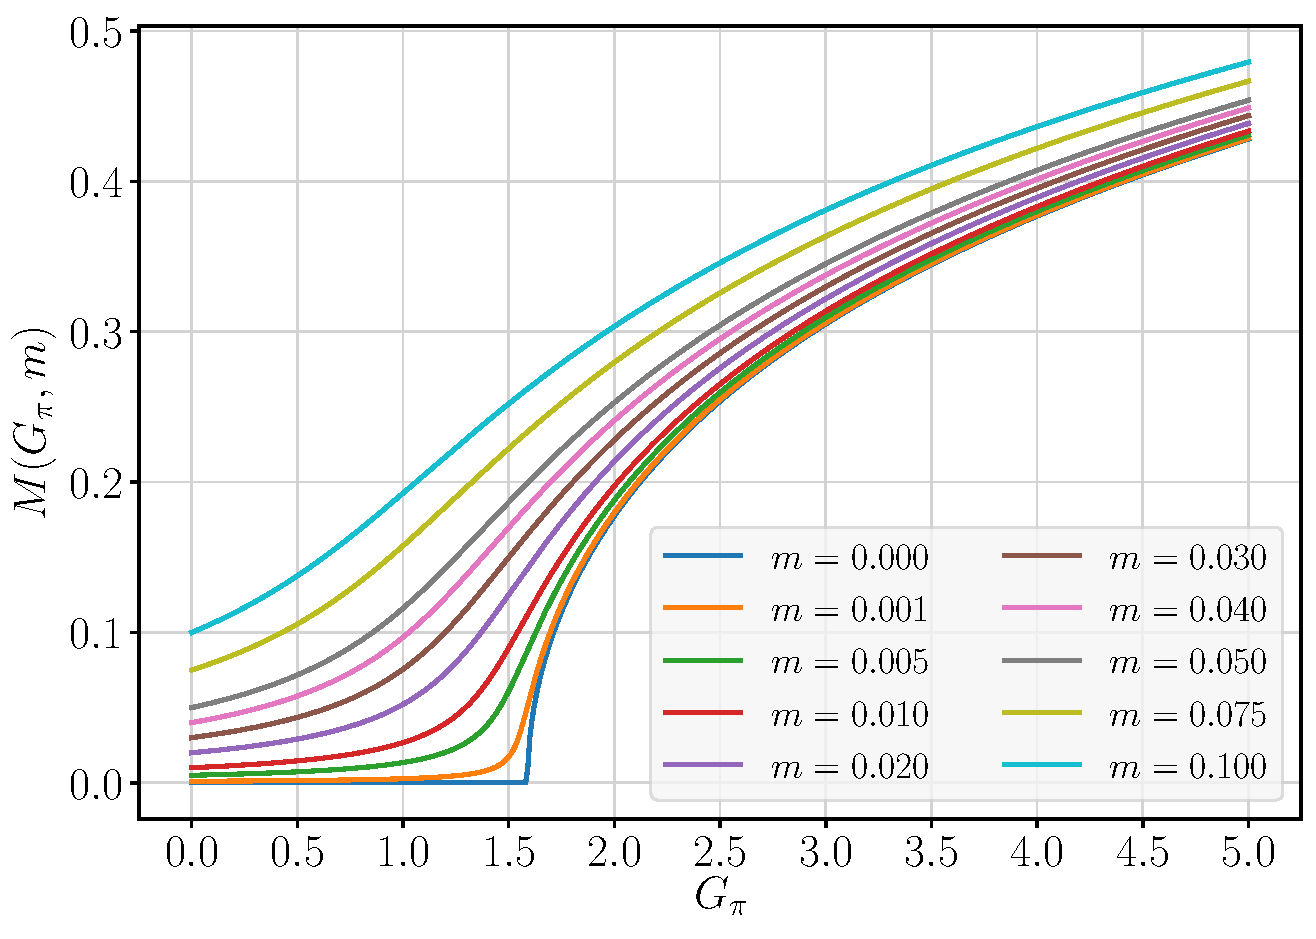
\includegraphics[width=.5\paperwidth]{Figures/chapter02/NJL-dressed-mass-curves}
	\end{center}

	\vspace{-1em}

	\begin{table}[!bp]
	  \centering
	  % \caption{Parameters used for solving the NJL model in $1+1$ dimensions.}
	  \label{tab:NJL1-analytical-solution-parameters}
	  \begin{tabular}{ c c c c c }
	    \hline
	    % \rule{0pt}{14pt}
	    $N_\text{Dirac}$ & $N_\text{color}$ & $N_\text{flavor}$ &
	    $\Lambda_{IR}$ & $\Lambda_{UV}$ \\
	    \hline
	    \hline
	    % \rule{0pt}{14pt}
	    $1+1 \ra 2$ & $1$ & $1$ & $0.240$ GeV & $0.645$ GeV \\
	    \hline
	  \end{tabular}
	\end{table}

\end{frame}


%% ----------------------------------------------------------------------------
%% LATTICE FORMULATION
%% ----------------------------------------------------------------------------

\subsection{Lattice formulation}

%% ----------------------------------------------------------------------------
%% ----------------------------------------------------------------------------

\begin{frame}[allowframebreaks]{Lattice formulation}

	We can define the Hamiltonian of the system as the integral over space of the Hamiltonian density:

	\begin{gather*}
		H = \int \mathcal{H}(x) \dd{x}
	    = \int \qty{
	      \bar{\psi}_{\alpha}(x)
	      \qty(\hat{m}_{\alpha\beta} - \delta_{\alpha\beta}i\gamma^{1}\partial_{1})
	      \psi_{\beta}(x) -
	      \frac{1}{2}G_{\pi}
	      \qty[\bar{\psi}_{\alpha}(x)\psi_{\alpha}(x)]^{2}} \dd{x}
	\end{gather*}

	For a basis where:

	\begin{gather*}
		\psi_{\alpha} = \mqty[\psi_{\alpha,+} \\ \psi_{\alpha,-}] \qc
	  \bar{\psi}_{\alpha} \defeq \psi^{\dagger}_{\alpha}\gamma^{0} \qc
		\gamma^{0} = \mqty[1 & 0\\ 0 & -1] \qc
	  \gamma^{1} = \mqty[0 & -1\\ 1 & 0]
	\end{gather*}

	Dropping the flavor indices to avoid clutter we can then write the kinetic term as:

	\begin{gather*}
	  \bar{\psi}\qty(-i\gamma^{1}\partial_{1})\psi =
			\frac{i}{2} \qty{
	      \qty[ \psi^{\dagger}_{+} \qty(\partial_{1}\psi_{-}) -
	      \qty(\partial_{1}\psi^{\dagger}_{+}) \psi_{-} ] +
	      \qty[ \psi^{\dagger}_{-} \qty(\partial_{1}\psi_{+}) -
	      \qty(\partial_{1}\psi^{\dagger}_{-}) \psi_{+} ]
	    }
	\end{gather*}

%% ----------------------------------------------------------------------------
\break
%% ----------------------------------------------------------------------------

	The two groups in brackets are essentially equivalent to one another by virtue of exchanging positive and negative energy components. This is the motivation behind \textbf{staggered fermion lattices}, which use two computational lattice sites for each theoretical value of $\psi$.

	\begin{figure}[!tbp]
		\centering
		\begin{minipage}[c]{.45\linewidth}
			\centering
			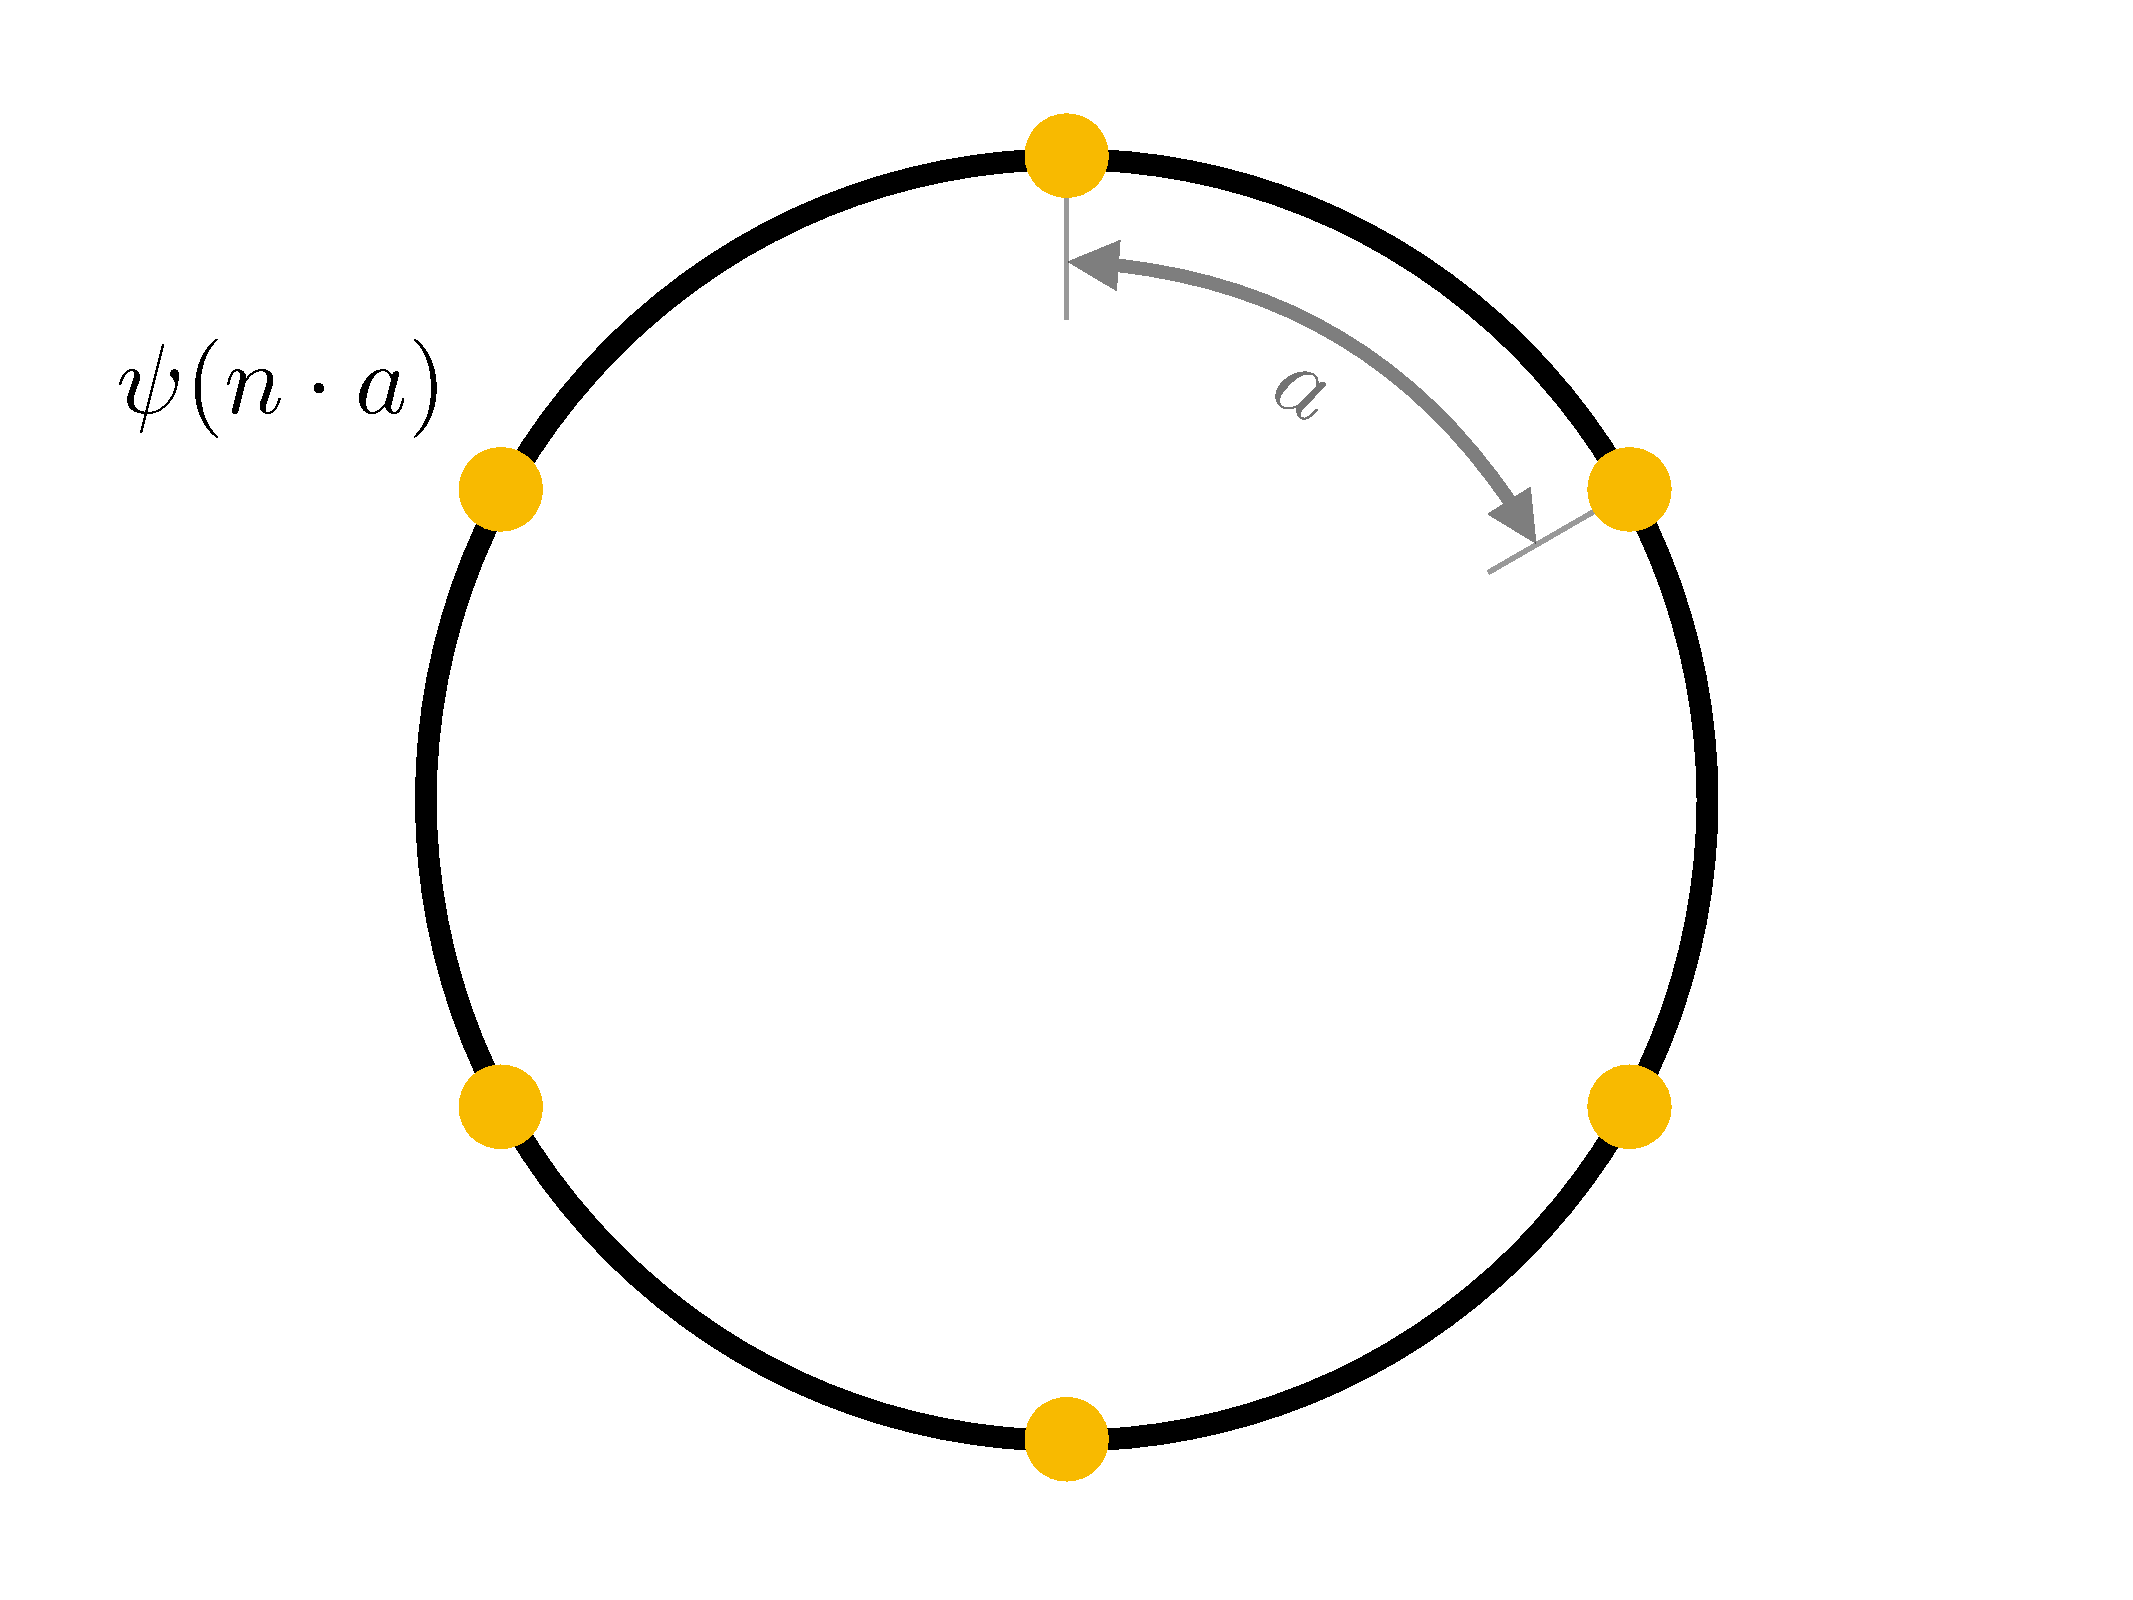
\includegraphics[width=\linewidth]{Figures/chapter02/physical-fermion-lattice}
		\end{minipage}
	  \hspace{.025\linewidth}
		\begin{minipage}[c]{.45\linewidth}
			\centering
			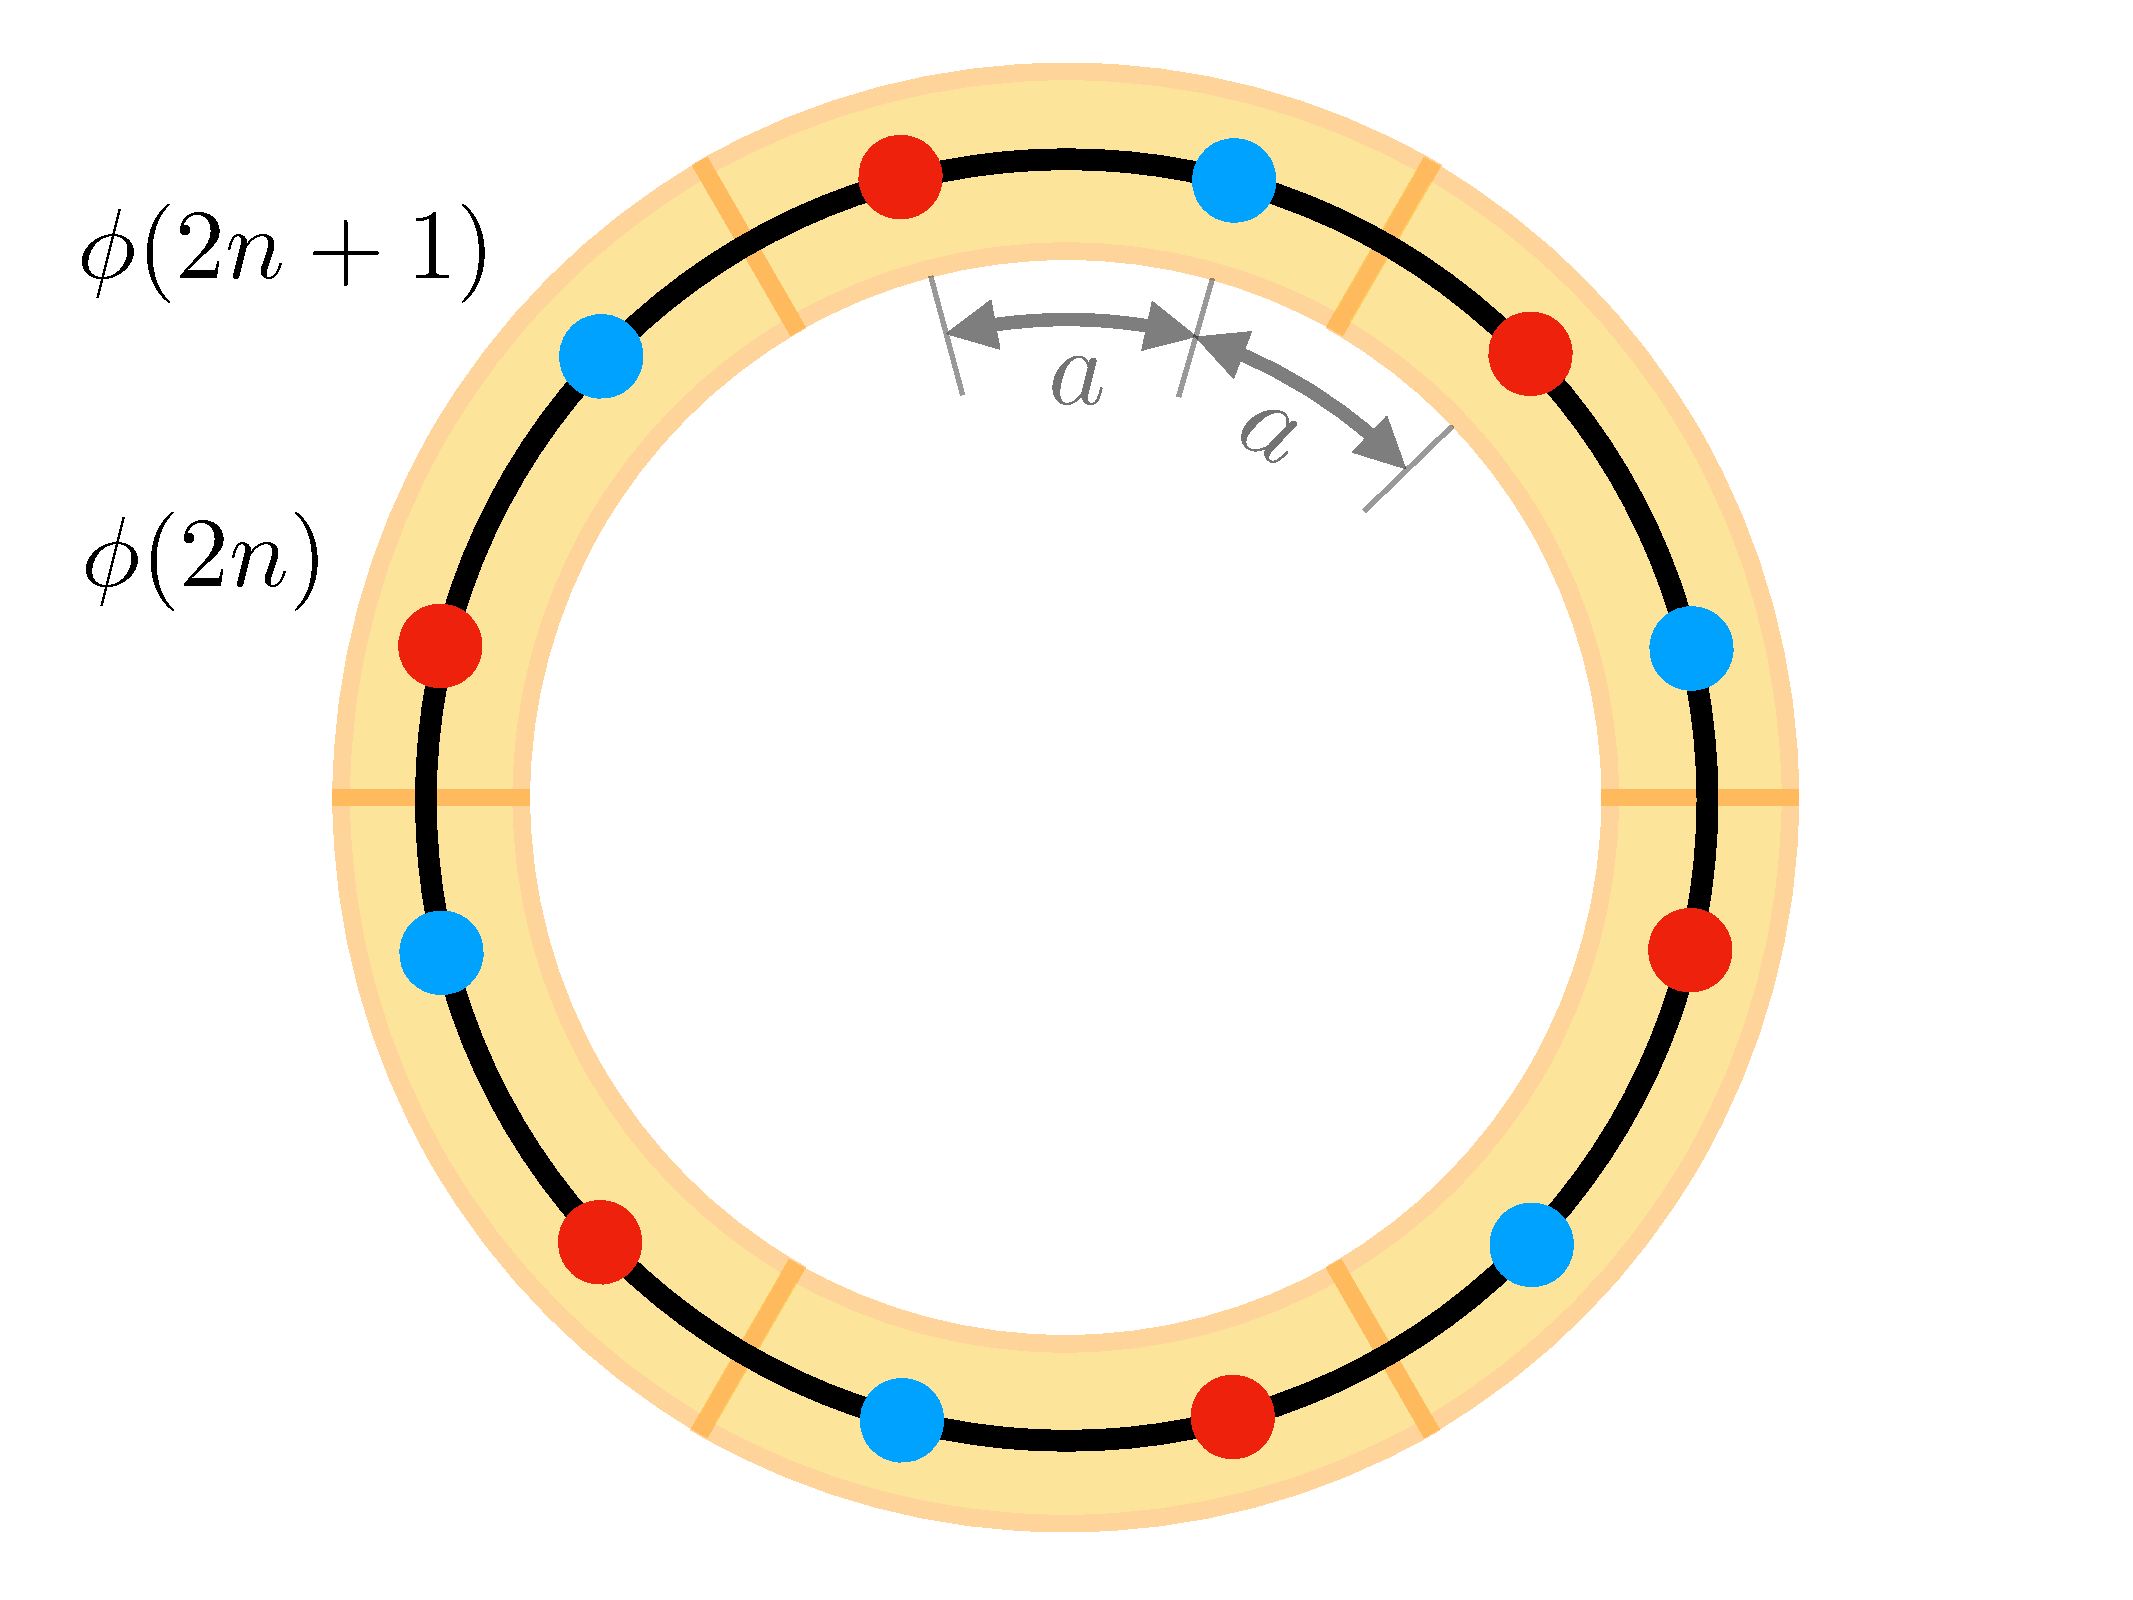
\includegraphics[width=\linewidth]{Figures/chapter02/computational-fermion-lattice}
		\end{minipage}
	\end{figure}

%% ----------------------------------------------------------------------------
\break
%% ----------------------------------------------------------------------------

	Sites in the staggered computational lattice are labeled using a parameter $n \in \mathds{Z}$ such that all evaluations of $\psi$ are made at integer multiples of the distance $a$:

	\begin{gather*}
	  \phi(n) \defeq \sqrt{a}
	    \begin{cases}
	      \psi_{+}\qty(\frac{n}{2}a) \qc &2 \mid n \\
	      \psi_{-}\qty(\frac{n-1}{2}a) \qc &2 \nmid n
	    \end{cases}
	\end{gather*}

	These newly defined operators obey the \textbf{canonical anti-commutation relations for fermions}:

	\begin{gather*} \label{eq:fermion-canonical-commutation-relations}
	  \acom{\phi^{\dagger}(p)}{\phi(q)} = \delta_{pq} \qc
	  \acom{\phi(p)}{\phi(q)} = 0
	\end{gather*}

	Finally, thanks to the periodic boundary conditions, we can write:

	\begin{gather*}
	  H_{N}^{(K)} =
	    \frac{i}{2a} \sum_{n=0}^{2N-1} \qty[
	    \phi^{\dagger}(n)\phi(n+1) - \phi^{\dagger}(n+1)\phi(n)]
	\end{gather*}

%% ----------------------------------------------------------------------------
\break
%% ----------------------------------------------------------------------------

	From this Hamiltonian, we can now recover the \textbf{masless Dirac equation} in the continuum limit; which serves as proof of correctness:

	\begin{gather*}
	  \dot{\phi}(n) =
      i\com{H_{N}^{(K)}}{\phi(n)} =
      \frac{\phi(n+1)-\phi(n-1)}{2a}
	\end{gather*}

	In terms of the original fields, this is:

	\begin{gather*}
	  \dot{\psi_{+}} = \frac{\Delta \psi_{-}}{\Delta x} \qc
	  \dot{\psi_{-}} = \frac{\Delta \psi_{+}}{\Delta x}
	\end{gather*}

	Lastly, taking the limit when $a \ra 0$:

	\begin{gather*}
	  \pderivative{t}\psi =
      \mqty[0 & 1 \\ 1 & 0] \pderivative{x}\psi \equiv
      \hat{\alpha}_1 \pderivative{x}\psi
	\end{gather*}

\end{frame}

%% ----------------------------------------------------------------------------
%% ----------------------------------------------------------------------------

\begin{frame}[allowframebreaks]{Multi-flavor lattice}

  To obtain the other components of the Hamiltonian from the expressions in the Hamiltonian density, which are written in terms of \textbf{Dirac bilinears}, we need to restore the flavor indices and deal with them in the computational lattice.

  \vspace{1em}
  Assuming that each flavor is independent, we could simply repeat the same procedure over different computational lattices and sum the results for all flavors. For instance, assuming that the \textbf{mass matrix is diagonal} (i.e. $\hat{m}_{\alpha\beta}=\text{diag}\qty[m_0,m_1,\ldots]$):

  \begin{align*}
  \int \bar{\psi}_{\alpha}\psi_{\alpha} \dd{x} \qra
    &\sum_{n=0}^{N-1}
      \qty[ \phi_{\alpha}^{\dagger}(2n)\phi_{\alpha}(2n) -
      \phi_{\alpha}^{\dagger}(2n+1)\phi_{\alpha}(2n+1) ] = \\
    &\sum_{n=0}^{2N-1} (-1)^{n}\phi_{\alpha}^{\dagger}(n)\phi_{\alpha}(n)
  \end{align*}

%% ----------------------------------------------------------------------------
\break
%% ----------------------------------------------------------------------------

  However the interaction will always introduce \textbf{cross-flavor terms} rendering this invalid:

  \begin{gather*}
  \int \qty(\sum_{\alpha}\bar{\psi}_{\alpha}\psi_{\alpha})^{2} \dd{x}
    \,=\,\,
    \int \qty[\sum_{\alpha} \qty(\bar{\psi}_{\alpha}\psi_{\alpha})^{2} +
    2\sum_{\alpha < \beta} \qty(\bar{\psi}_{\alpha}\psi_{\alpha})
    \qty(\bar{\psi}_{\beta}\psi_{\beta})] \dd{x}
  \end{gather*}

  To solve this, we will build a single computational lattice with all the components of the field associated to different flavors stitched together back-to-back. The resulting operators are:

  \begin{gather*}
  \phi_{\alpha}(n) \equiv \phi(n + 2N\alpha) \defeq \sqrt{a}
    \begin{cases}
      \psi_{\alpha,+}\qty(\frac{n}{2}a) \qc &2 \mid n \\
      \psi_{\alpha,-}\qty(\frac{n-1}{2}a) \qc &2 \nmid n
    \end{cases} \\[1em]
    \acom{\phi_{\alpha}^{\dagger}(p)}{\phi_{\beta}(q)} =
      \delta_{\alpha\beta}\delta_{pq} \qc
    \acom{\phi_{\alpha}(p)}{\phi_{\beta}(q)} = 0
  \end{gather*}

%% ----------------------------------------------------------------------------
\break
%% ----------------------------------------------------------------------------

  With \textbf{periodic boundary conditions} applied on each flavor separately (i.e. not crossing over to other flavors $\phi_\alpha(2N) = \phi_\alpha(0) \neq \phi_{\alpha+1}(0)$).

  \begin{figure}[!tbp]
    \centering
    \begin{minipage}[c]{.45\linewidth}
      \centering
      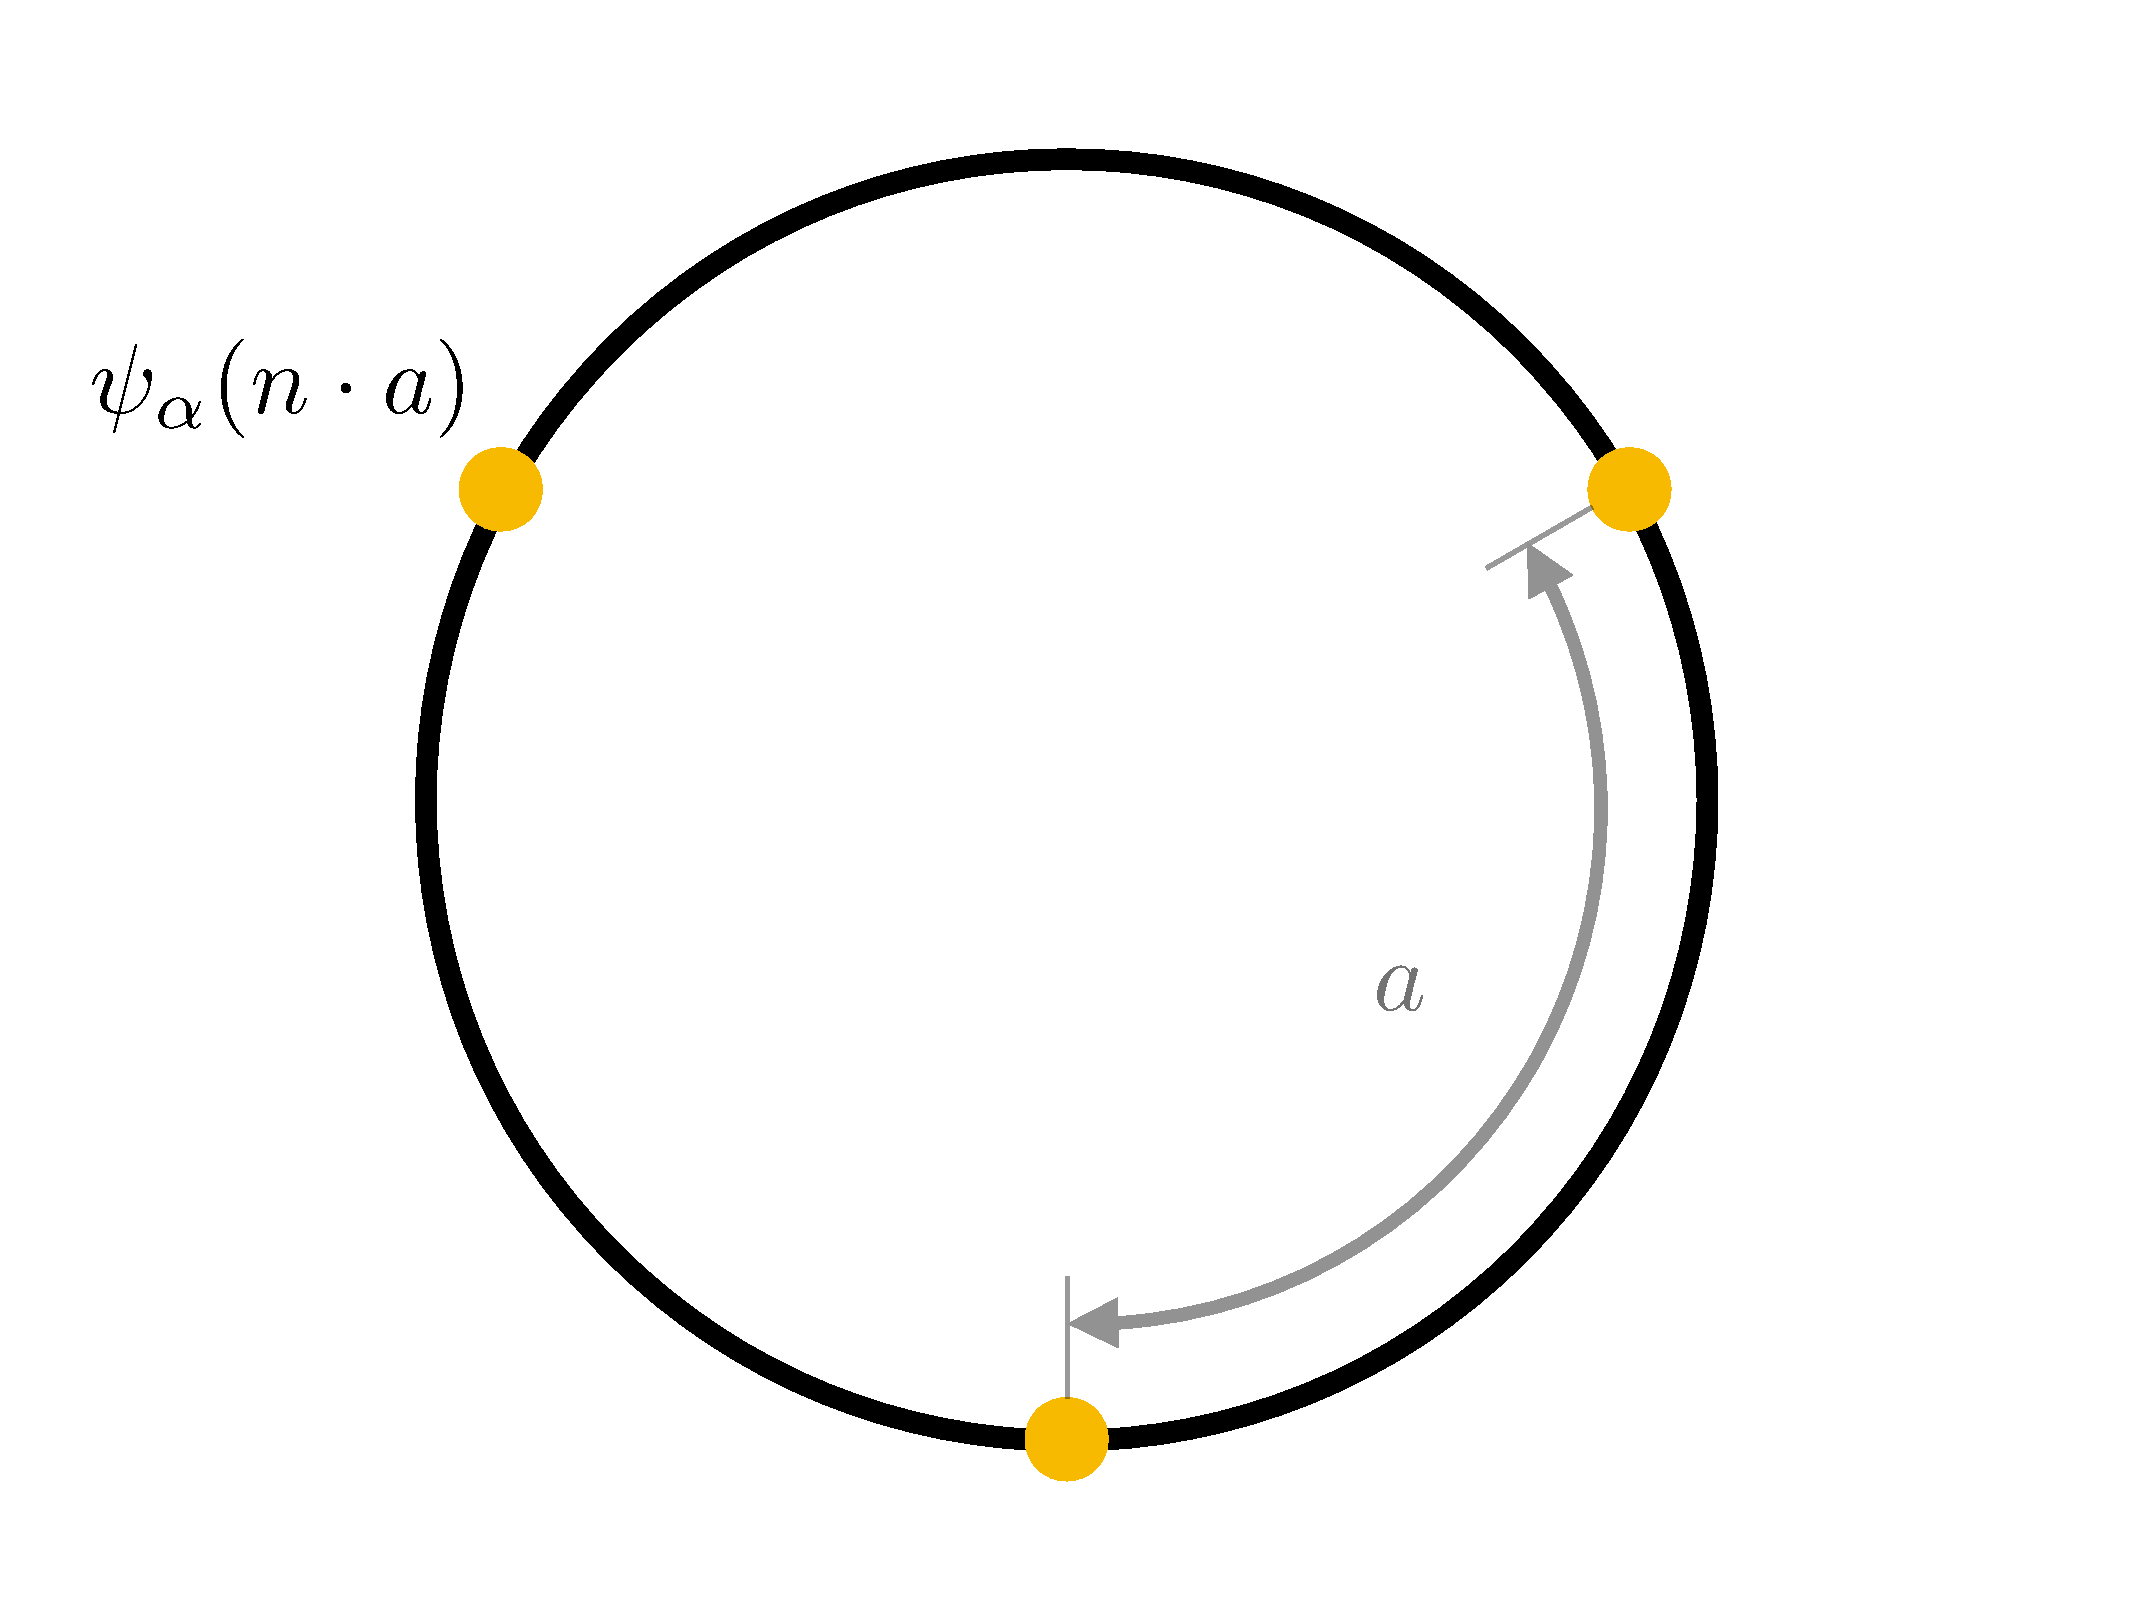
\includegraphics[width=\linewidth]{Figures/chapter02/physical-fermion-lattice-flavor}
    \end{minipage}
    \hspace{.025\linewidth}
    \begin{minipage}[c]{.45\linewidth}
      \centering
      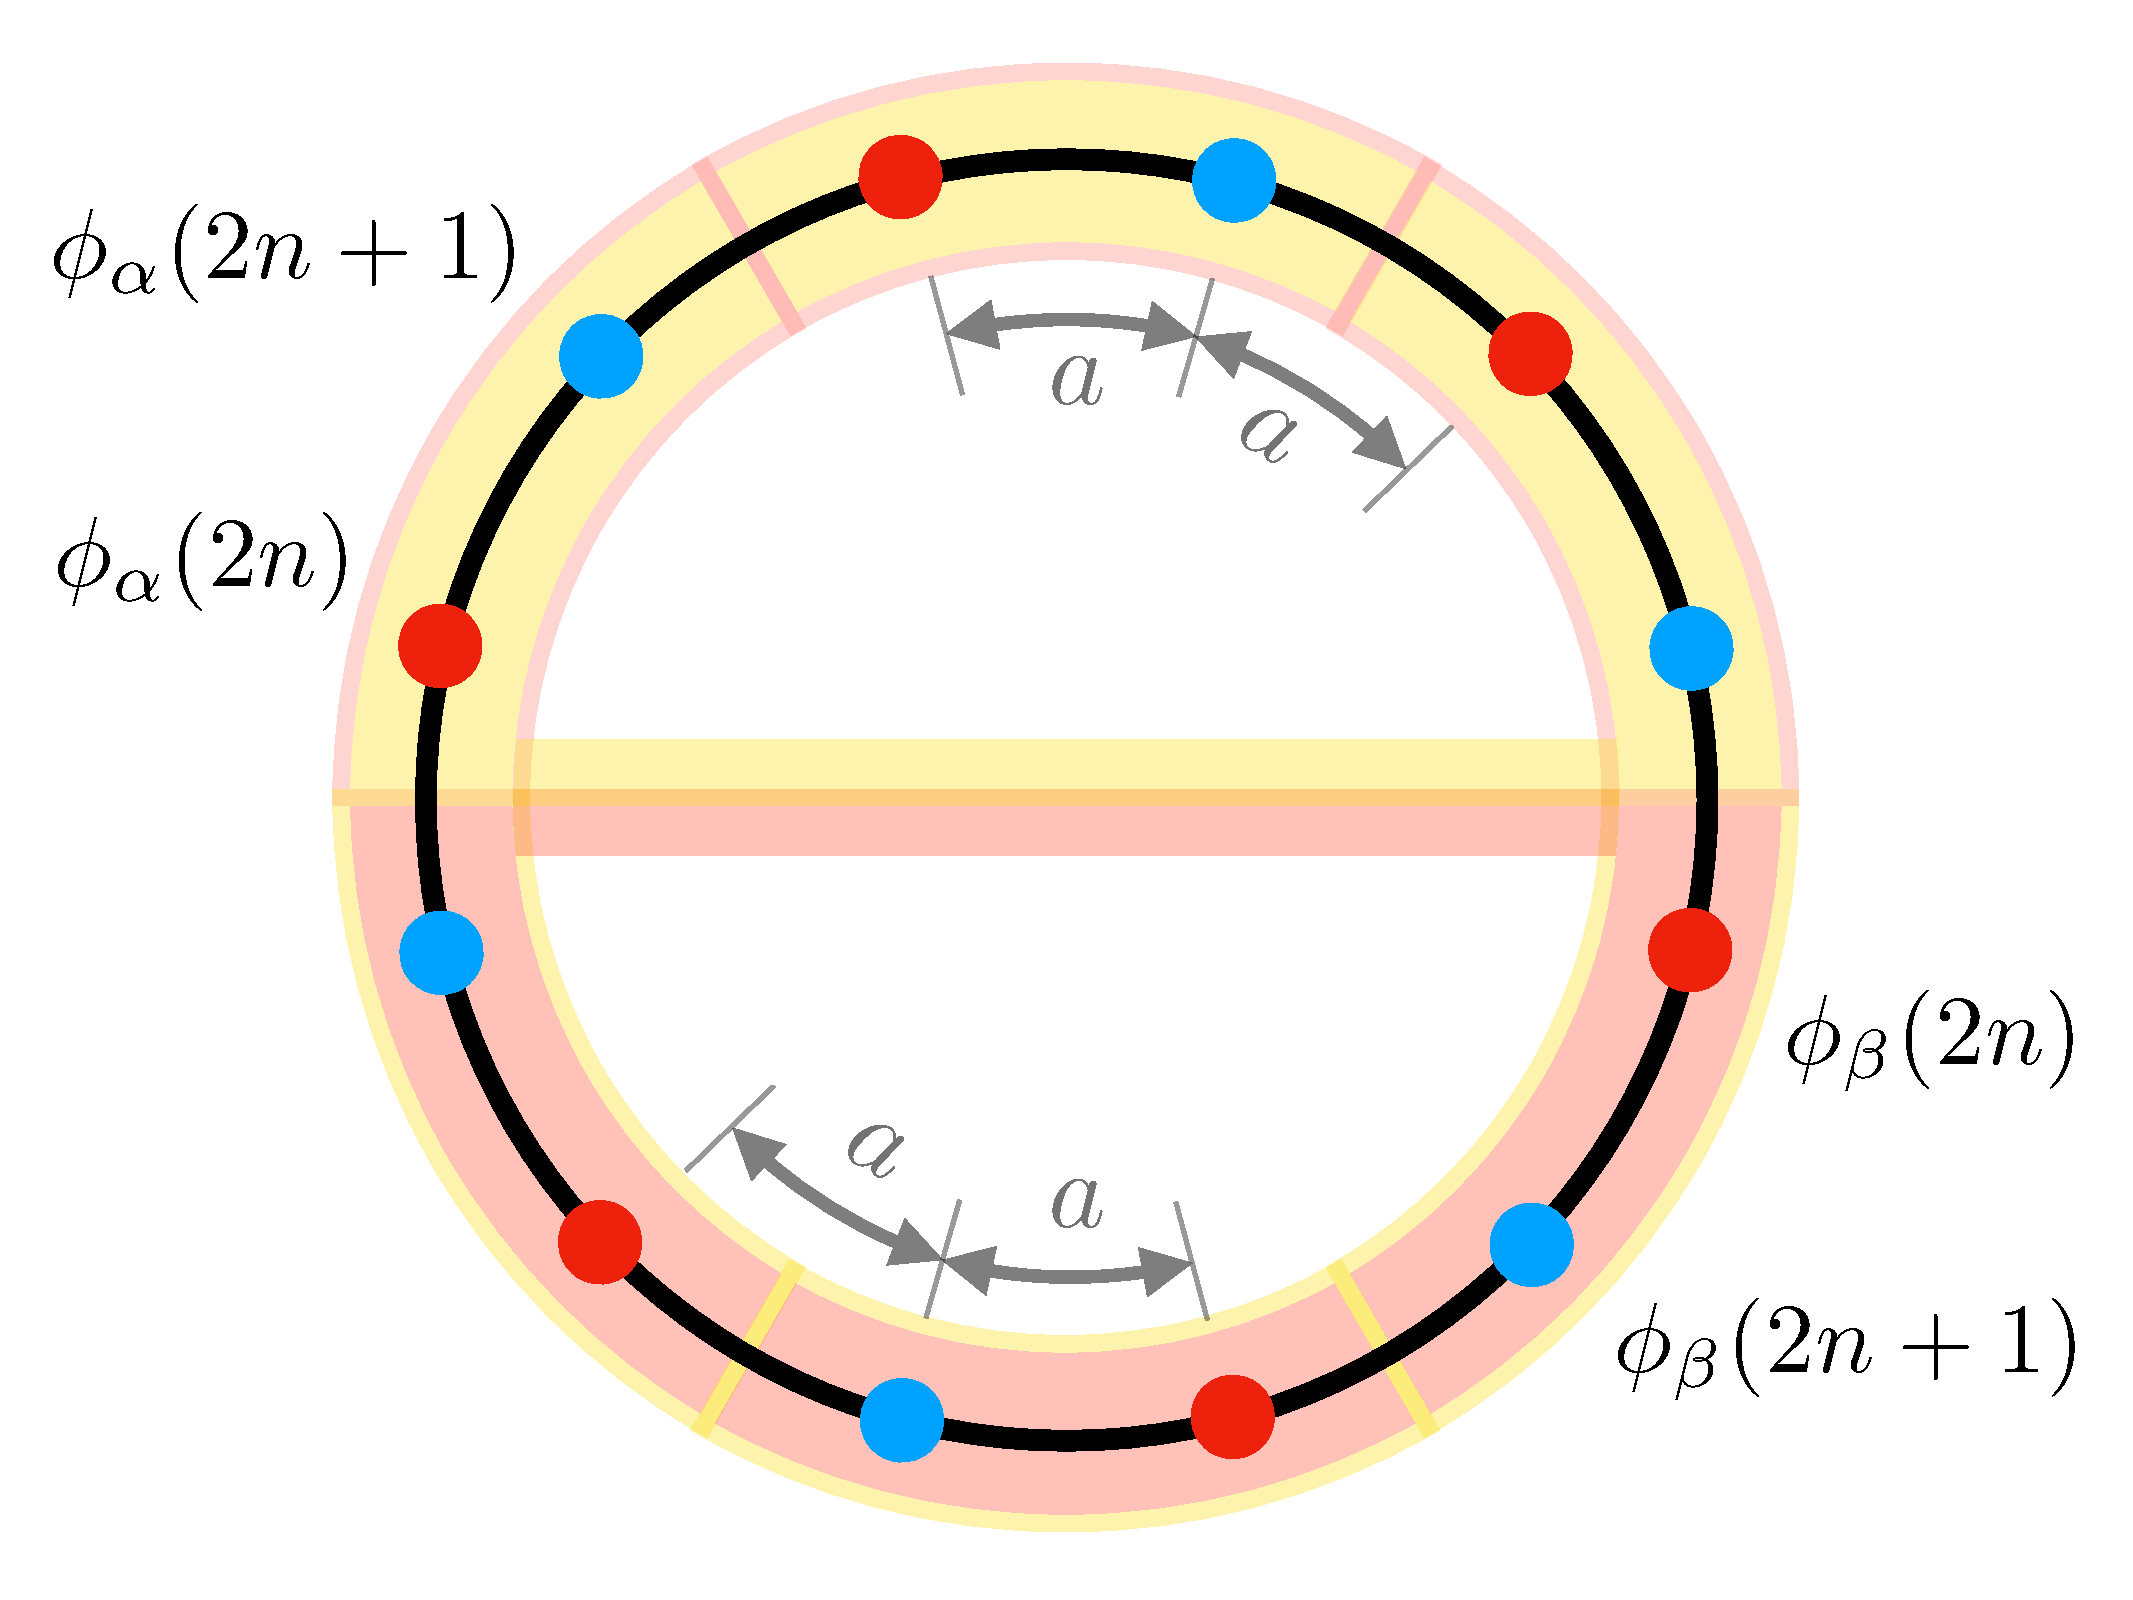
\includegraphics[width=\linewidth]{Figures/chapter02/computational-fermion-lattice-flavor}
    \end{minipage}
  \end{figure}

%% ----------------------------------------------------------------------------
\break
%% ----------------------------------------------------------------------------

  All in all, we obtain the following discretized NJL Hamiltonian for $1+1$ dimensions, any number of flavors $N_\text{flavor}$, $N$ physical lattice sites, and $2N\!\cdot\!N_\text{flavor}$ computational lattice sites:

  \begin{align*}
    H_{N} =&\, H_{N}^{(M)} + H_{N}^{(K)} + H_{N}^{(G)} \\
    H_{N}^{(M)} =&\,
      \sum_{\alpha} \sum_{n=0}^{2N-1}
      (-1)^{n} \, m_{\alpha} \phi_{\alpha}^{\dagger}(n)\phi_{\alpha}(n)  \\
    H_{N}^{(K)} =&\, \frac{i}{2a}
      \sum_{\alpha} \sum_{n=0}^{2N-1} \qty[
      \phi_{\alpha}^{\dagger}(n) \phi_{\alpha}(n+1) -
      \phi_{\alpha}^{\dagger}(n+1) \phi_{\alpha}(n)]  \\
    H_{N}^{(G)} =&\, - \frac{G_{\pi}}{2a} \sum_{n=0}^{N-1} \qty[
      \sum_{\alpha} \dbtilde{H}_{N}^{\alpha\alpha}(n) + 2
      \sum_{\alpha < \beta} \dbtilde{H}_{N}^{\alpha\beta}(n)]
  \end{align*}
  \begin{align*}
    \dbtilde{H}_{N}^{\alpha\beta}(n) \defeq&\,
      \qty[\phi_{\alpha}^{\dagger}(2n)\phi_{\alpha}(2n) -
      \phi_{\alpha}^{\dagger}(2n+1)\phi_{\alpha}(2n+1)] \times
      \qty[\phi_{\beta}^{\dagger}(2n)\phi_{\beta}(2n) -
      \phi_{\beta}^{\dagger}(2n+1)\phi_{\beta}(2n+1)]
  \end{align*}

\end{frame}
